\subsubsection{External Interface Requirements}

\subsubsection{User Interfaces}
qui ci vanno tutti i mockups con descrizione

\subsubsection{Hardware Interfaces}
The application does not need any specific hardware requirements. 

\subsubsection{Software Interfaces}
The web app requires a computer with a web browser installed and connected to 
The system has to rely on a DBMS API. It allows the management of all the data the system 
needs in order to provide its functionalities, described in subsection ~\ref{subsection:2.2}.

\subsubsection{Communication Interfaces}
All the communications between users and Dream website are made via HTTPS.

\newpage

\subsection{Functional Requirements}
\subsubsection{Use Case Diagram}
\begin{figure}[H]
    \begin{center}
    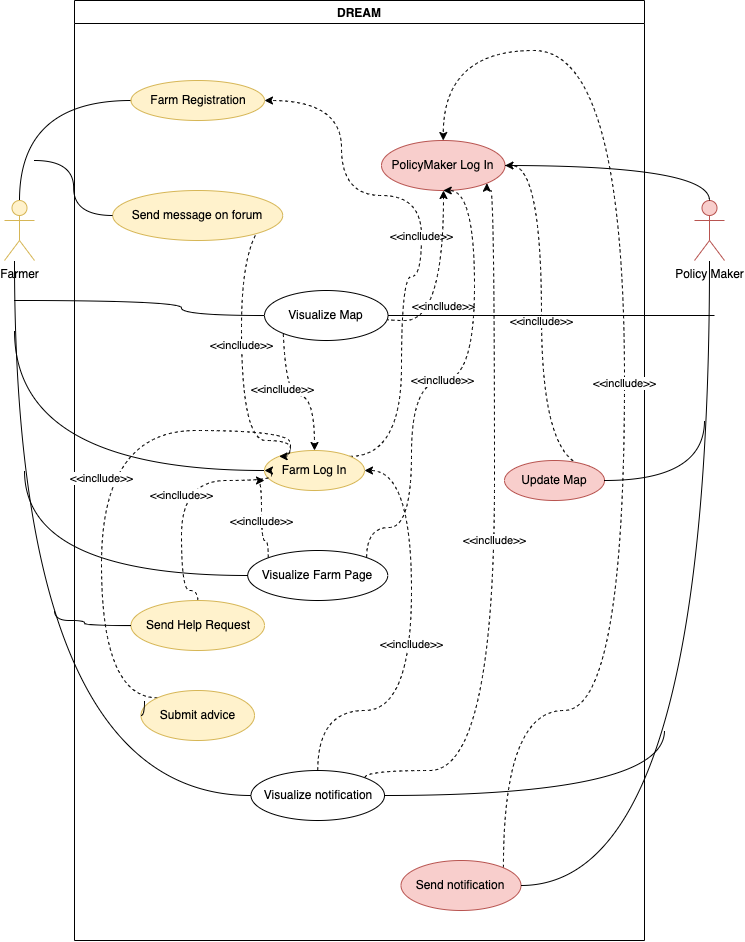
\includegraphics[width=1\textwidth]{images/useCaseDiag.drawio.png}
    \caption{Use Case diagram.}
    \label{fig:state9}
    \end{center}
\end{figure}
\subsubsection{Use Cases Description ad Sequence Diagram}
\begin{enumerate}
    \item \textbf{Farmer Registration} 
        \begin{longtable}{p{0.26\linewidth}p{0.75\linewidth}}
            \toprule
            \textbf{Name} & \textbf{Farmer Registration} \\
            \midrule
            \textbf{Actors} & Farmer \\
            \midrule
            \textbf{Entry conditions} & The web application has started\\
            \midrule
            \textbf{Flow of events} & 
            \begin{enumerate}
                \item The farmer wants to sign up
                \item The farmer inserts email, name, password, farm's name and farm's position 
                \item The farmer clicks submit
                \item The system checks if email is unique and if all the form is correctly fill up 
                \item The system inserts the information in the data base
            \end{enumerate} \\
            \midrule
            \textbf{Exit conditions} & The farmer is signed up\\
            \midrule
            \textbf{Exceptions} & 
            \begin{itemize}
                \item If the farmer did not insert data correctly the system will send an alert and let the user do that again
                \item If the email is already present in the database the system will send an alert saying that the email already exists
            \end{itemize} \\
            \bottomrule
            \caption{\emph{Farmer Registration} use case description}
        \end{longtable}
        
            \begin{figure}[H]
                \begin{center}
                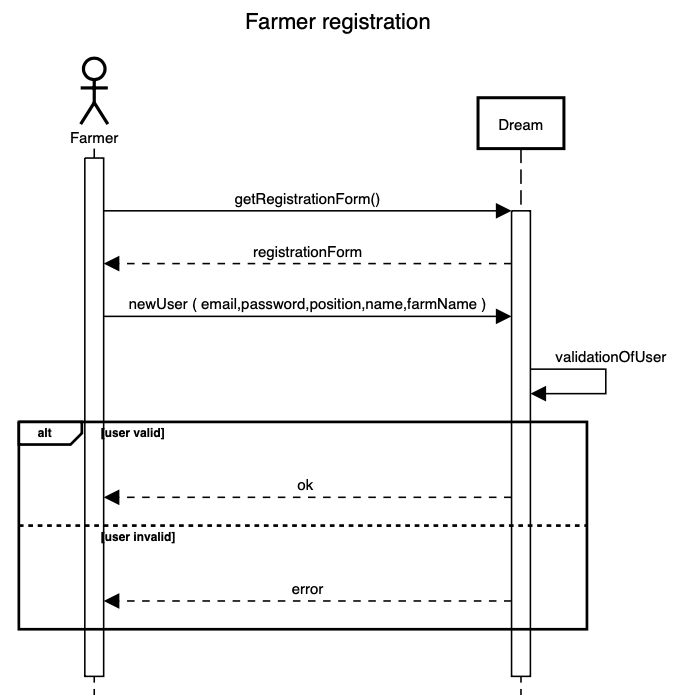
\includegraphics[width=0.7\textwidth]{sequence/FarmerRegistration.png}
                \caption{\emph{Farmer Registration} sequence diagram}
                \label{fig:sequence1}
                \end{center}
            \end{figure}

        \item \textbf{Farmer Login}
        \begin{longtable}{p{0.26\linewidth}p{0.75\linewidth}}
            \toprule
            \textbf{Name} & \textbf{Farmer Login} \\
            \midrule
            \textbf{Actors} & Farmer \\
            \midrule
            \textbf{Entry conditions} & The web application has started\\
            \midrule
            \textbf{Flow of events} & 
            \begin{enumerate}
                \item The farmer wants to log in
                \item The farmer inserts email and password
                \item The farmer clicks submit
                \item The system checks if the credentials are correct
                \item The system notifies the farmer about the correct login
            \end{enumerate} \\
            \midrule
            \textbf{Exit conditions} & The farmer has logged in\\
            \midrule
            \textbf{Exceptions} & 
            \begin{itemize}
                \item If the system does not recognize the email it will send and alert to the farmer saying that the email inserted is wrong
                \item If the password is not correct the system will notify the farmer
            \end{itemize} \\
            \bottomrule
            \caption{\emph{Farmer Login} use case description}
        \end{longtable}
        
        \begin{figure}[H]
        \begin{center}
        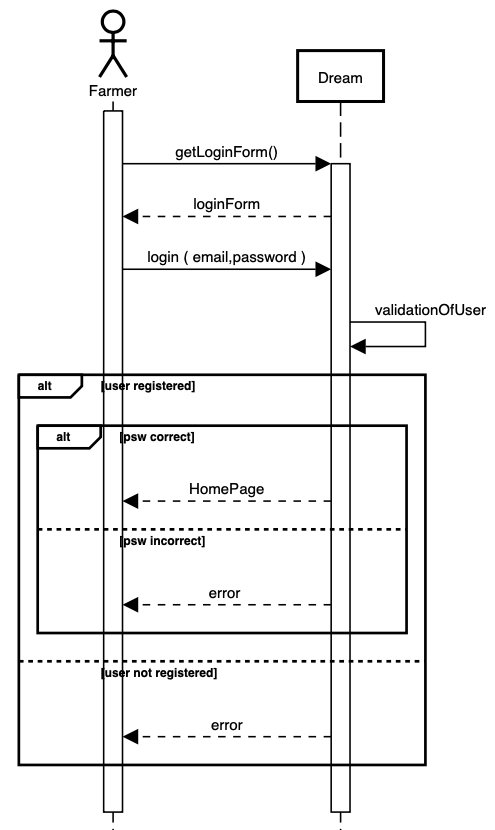
\includegraphics[width=0.5\textwidth]{sequence/FarmerLogin.png}
        \caption{\emph{Farmer Login} sequence diagram}
        \label{fig:sequence2}
        \end{center}
        \end{figure}


        \item Farmer send a message on the Forum
        \item \begin{longtable}{p{0.26\linewidth}p{0.75\linewidth}}
            \toprule
            \textbf{Name} & \textbf{Farmer sends a message on the forum} \\
            \midrule
            \textbf{Actors} & Farmer \\
            \midrule
            \textbf{Entry conditions} & The farmer has logged in\\
            \midrule
            \textbf{Flow of events} & 
            \begin{enumerate}
                \item The farmer wants to send a message
                \item The farmer clicks on forum button
                \item The system send the ser to the forum page
                \item The farmer inserts the message 
                \item The farmer clicks on send message
                \item The system inserts the message into the database 
            \end{enumerate} \\
            \midrule
            \textbf{Exit conditions} & The farmer's message is published\\
            \midrule
            \textbf{Exceptions} & 
            \begin{itemize}
                \item If the message body is empty the system shows an error alert
            \end{itemize} \\
            \bottomrule
            \caption{\emph{Farmer message} use case description}
        \end{longtable}
        \begin{figure}[H]
            \begin{center}
            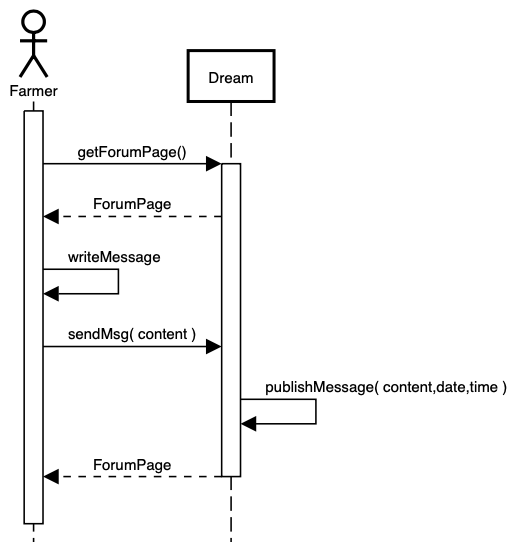
\includegraphics[width=0.6\textwidth]{sequence/messageOnForum.png}
            \caption{\emph{Farmer message} sequence diagram}
            \label{fig:sequence3}
        \end{center}
        \end{figure}

    \item Find a farmer on the Map\\
    \begin{longtable}{p{0.26\linewidth}p{0.75\linewidth}}
        \toprule
        \textbf{Name} & \textbf{Farmer visualizes the map} \\
        \midrule
        \textbf{Actors} & Farmer \\
        \midrule
        \textbf{Entry conditions} & The farmer has logged in\\
        \midrule
        \textbf{Flow of events} & 
        \begin{enumerate}
            \item The farmer wants to visualize the map
            \item The farmer clicks on map button
            \item The system send the farmer to the map page
            \item The farmer visualizes the map and selects a farm
            \item The system retrieves the information about the farm and shows them to the farmer
            \item The farmer visualizes the data about the selected farm
        \end{enumerate} \\
        \midrule
        \textbf{Exit conditions} & The farmer visualized the map\\
        \midrule
        \textbf{Exceptions} & \\
        \bottomrule
        \caption{\emph{Farms' map visualization} use case description}
    \end{longtable}
    \begin{figure}[H]
        \begin{center}
        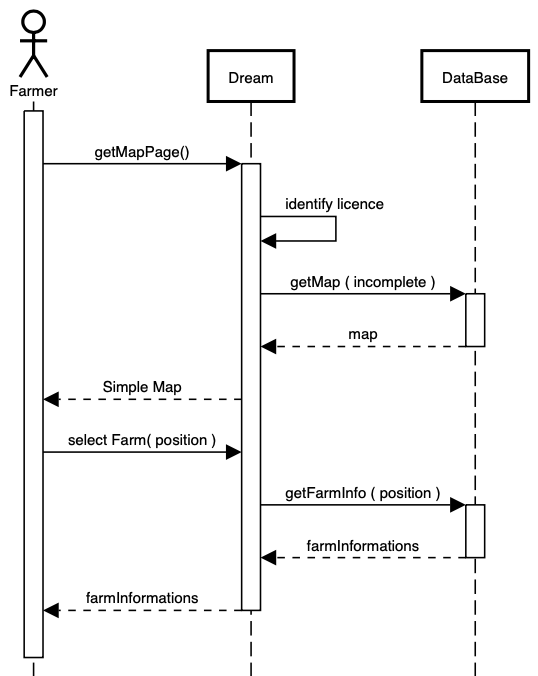
\includegraphics[width=0.45\textwidth]{sequence/VisializeMap.png}
        \caption{\emph{Farms' map visualization} sequence diagram}
        \label{fig:sequence4}
        \end{center}
    \end{figure}
    
    \item Find farm’s information
    \begin{longtable}{p{0.26\linewidth}p{0.75\linewidth}}
        \toprule
        \textbf{Name} & \textbf{Farmer visualizes their own data} \\
        \midrule
        \textbf{Actors} & Farmer \\
        \midrule
        \textbf{Entry conditions} & The farmer has logged in\\
        \midrule
        \textbf{Flow of events} & 
        \begin{enumerate}
            \item The farmer wants to visualize his own page
            \item The farmer clicks on the profile page button
            \item The system retrives the information about the farmer and redirect him to the farmer's farm page
            \item The farmer visualize his own page
        \end{enumerate} \\
        \midrule
        \textbf{Exit conditions} & The farmer visualizes his own data\\
        \midrule
        \textbf{Exceptions} & 
        \begin{enumerate}
            \item
        \end{enumerate}\\
        \bottomrule
        \caption{\emph{Farm information visualization} use case description}
    \end{longtable}
    \begin{figure}[H]
        \begin{center}
        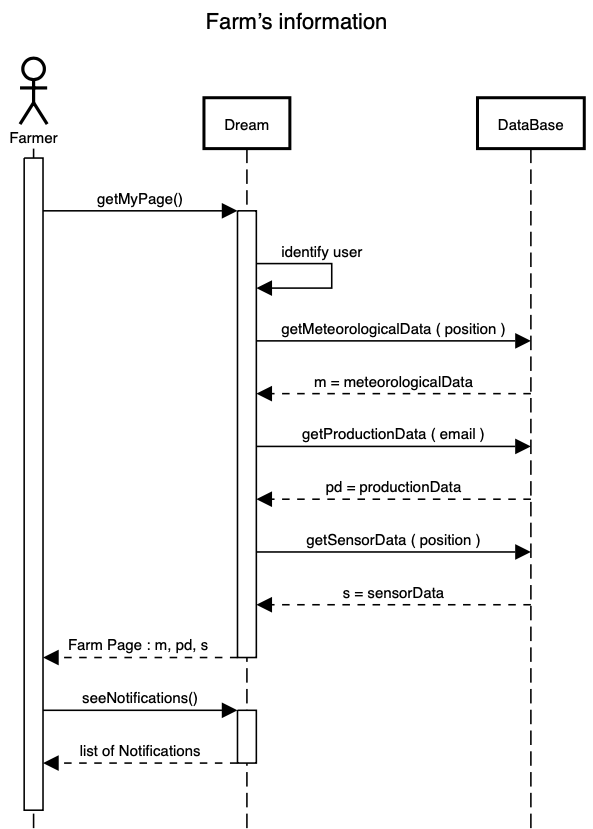
\includegraphics[width=0.7\textwidth]{sequence/FarmInformation.png}
        \caption{\emph{Farm information visualization} sequence diagram}
        \label{fig:sequence5}
        \end{center}
    \end{figure}

    \item Submit a request of help\\
    \textbf{I put only the case of a forml request to the Policy Maker (button on Farm Page) if you want we can create 2 "secion" (alt) one with this formal request and one sending a message on Forum (but is yet specified in 3)}
    \begin{longtable}{p{0.26\linewidth}p{0.75\linewidth}}
        \toprule
        \textbf{Name} & \textbf{Farmer submit a request of help} \\
        \midrule
        \textbf{Actors} & Farmer \\
        \midrule
        \textbf{Entry conditions} & The farmer has logged in\\
        \midrule
        \textbf{Flow of events} & 
        \begin{enumerate}
            \item The farmer wants to ask for help
            \item The farmer clicks on his own page button
            \item The farmer clicks on Help button
            \item The farmer chooses the type of production on which he had problems
            \item The farmer fill the form specifying the problem in details
            \item The farmer click on submit button and send the message
            \item The system send the notification to the Policy Makers
            \item The system notifies the farmer that the operation went succesfully
            \item The system returns a list of advices found in the database about this type of production
        \end{enumerate} \\
        \midrule
        \textbf{Exit conditions} & The help request is send to the Policy Makers\\
        \midrule
        \textbf{Exceptions} & 
        \begin{itemize}
            \item If no type of production is selected the system notifies the farmer and waits for him to insert it
            \item If the request body is empty the system notifies the farmer and waits for him to fill it
        \end{itemize}\\
        \bottomrule
        \caption{\emph{Farmer ask for help} use case description}
    \end{longtable}
    \begin{figure}[H]
        \begin{center}
        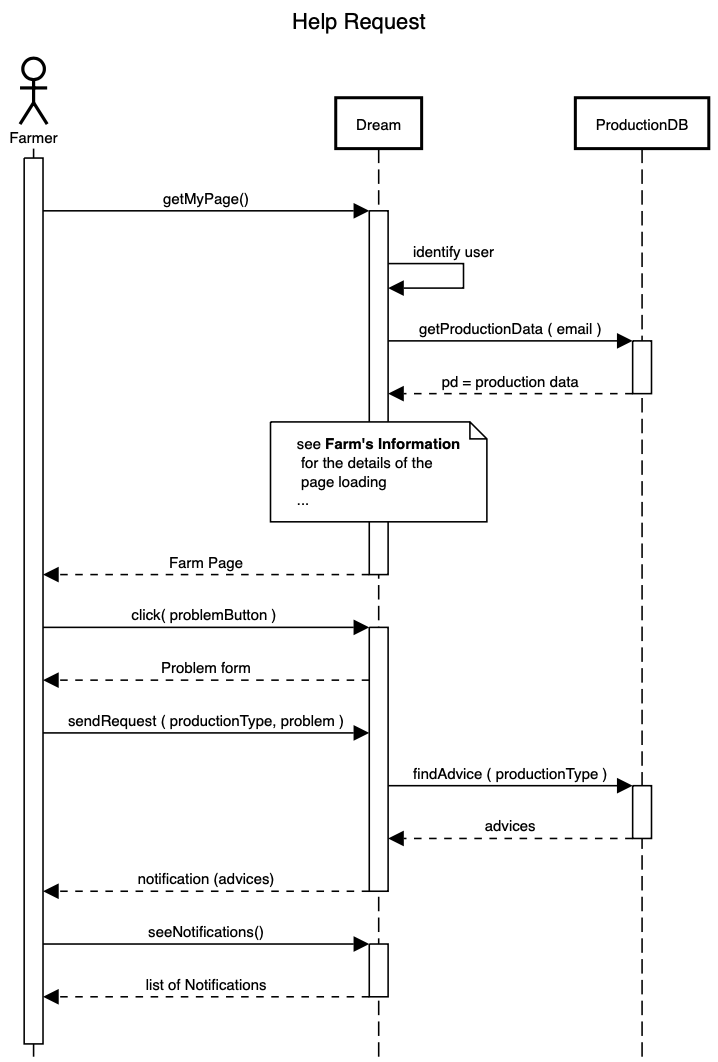
\includegraphics[width=0.7\textwidth]{sequence/HelpRequest.png}
        \caption{\emph{Farmer ask for help} sequence diagram}
        \label{fig:sequence6}
        \end{center}
    \end{figure}

    \item Submit an advice
    \begin{longtable}{p{0.26\linewidth}p{0.75\linewidth}}
        \toprule
        \textbf{Name} & \textbf{Farmer submit an advice} \\
        \midrule
        \textbf{Actors} & Farmer \\
        \midrule
        \textbf{Entry conditions} & The farmer has logged in\\
        \midrule
        \textbf{Flow of events} & 
        \begin{enumerate}
            \item The farmer has to submit an advice 
            \item The farmer clicks on his own page button
            \item The farmer clicks on Advice button
            \item The farmer chooses the type of production on which he wants to gave advices
            \item The farmer fill the form writing his advice
            \item The farmer clicks submit button and send the message
            \item The system save the advice in the database
            \item The system notifies the farmer that the operation went succesfully 
        \end{enumerate} \\
        \midrule
        \textbf{Exit conditions} & The farmer submit an advice\\
        \midrule
        \textbf{Exceptions} & 
        \begin{itemize}
            \item If the farmer is not a "good" one the system don't save the advice and notice him whith an error message
        \end{itemize}\\
        \bottomrule
        \caption{\emph{Farmer send advice} use case description}
    \end{longtable}
    \begin{figure}[H]
        \begin{center}
        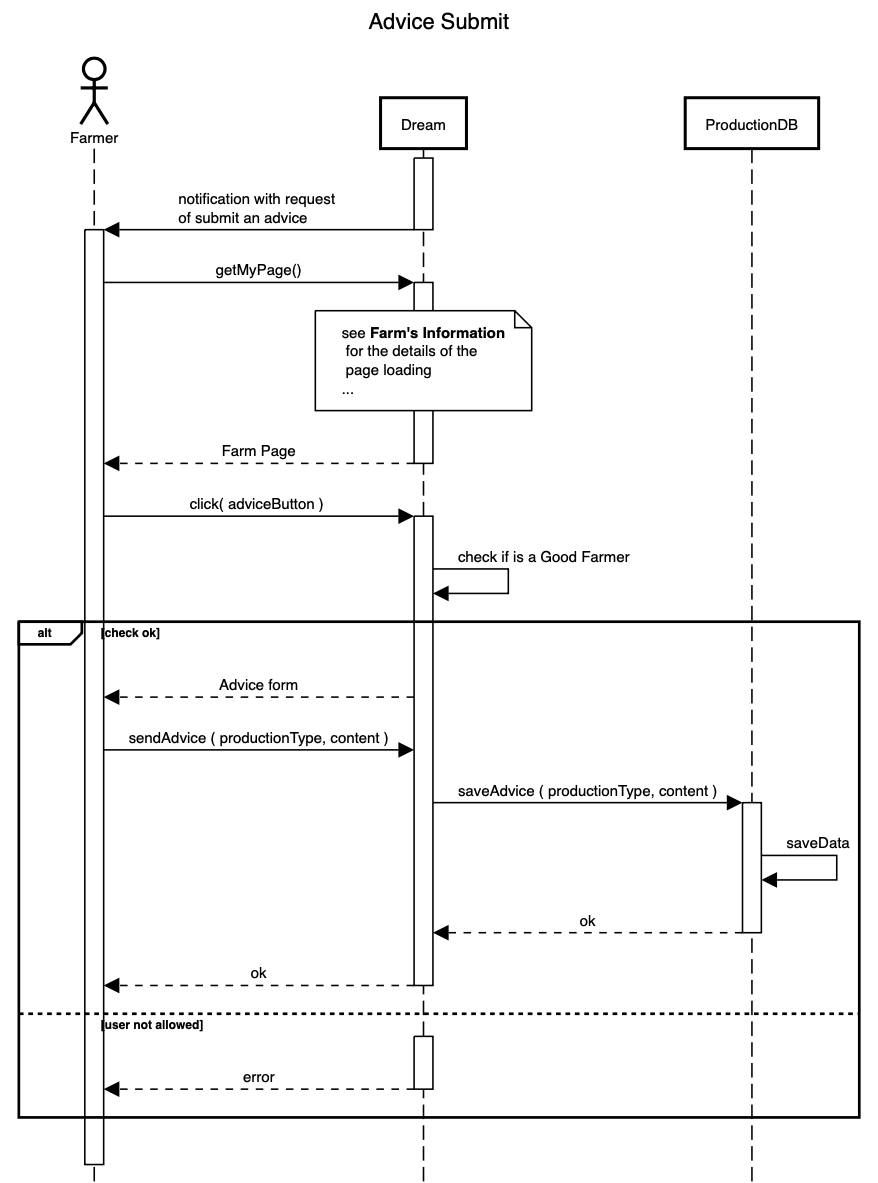
\includegraphics[width=0.7\textwidth]{sequence/AdviceSubmit.png}
        \caption{\emph{Farmer send advice} sequence diagram}
        \label{fig:sequence7}
        \end{center}
    \end{figure}

    \item Visualize notifications
    \begin{longtable}{p{0.26\linewidth}p{0.75\linewidth}}
        \toprule
        \textbf{Name} & \textbf{Farmer visualizes his notifications} \\
        \midrule
        \textbf{Actors} & Farmer \\
        \midrule
        \textbf{Entry conditions} & The farmer has logged in\\
        \midrule
        \textbf{Flow of events} & 
        \begin{enumerate}
            \item The farmer wants to reads his notifications
            \item The farmer clicks on his own page button
            \item The farmer clicks on Notification button
            \item The system returns a list of messages
            \item The farmer select one message between the ones in the list
            \item The system return the body of the message
        \end{enumerate} \\
        \midrule
        \textbf{Exit conditions} & The farmer visualizes his notifications\\
        \midrule
        \textbf{Exceptions} & 
        \begin{itemize}
            \item 
        \end{itemize}\\
        \bottomrule
        \caption{\emph{Farmer visualize notifications} use case description}
    \end{longtable}
    \begin{figure}[H]
        \begin{center}
        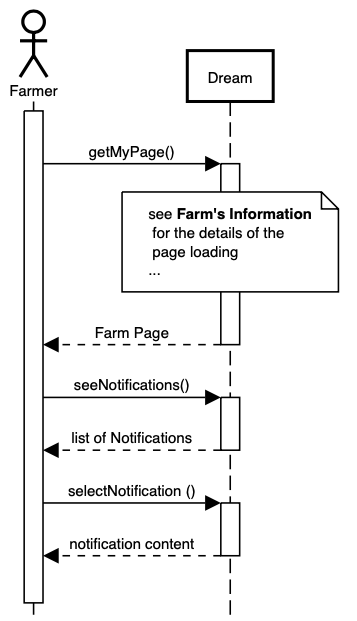
\includegraphics[width=0.7\textwidth]{sequence/SeeNotifications.png}
        \caption{\emph{Farmer visualize notifications} sequence diagram}
        \label{fig:sequence8}
        \end{center}
    \end{figure}

    \item Policy Maker login
    \begin{longtable}{p{0.26\linewidth}p{0.75\linewidth}}
        \toprule
        \textbf{Name} & \textbf{Farmer visualizes their own data} \\
        \midrule
        \textbf{Actors} & Policy Maker \\
        \midrule
        \textbf{Entry conditions} & The web application has started\\
        \midrule
        \textbf{Flow of events} & 
        \begin{enumerate}
            \item The Policy Maker wants to log in 
            \item The Policy Maker inserts code and password
            \item The Policy Maker clicks submit button
            \item The system checks if the credentials are correct
            \item The system notifies the Policy Maker about the correct login
        \end{enumerate} \\
        \midrule
        \textbf{Exit conditions} & The Policy Maker has logged in\\
        \midrule
        \textbf{Exceptions} & 
        \begin{itemize}
            \item If the system does not recognize the code it will send and alert the Policy Maker saying the code inserted is wrong
            \item If the password is not correct the system will notify the Policy Maker 
        \end{itemize}\\
        \bottomrule
        \caption{\emph{Policy Maker login} use case description}
    \end{longtable}
    \begin{figure}[H]
        \begin{center}
        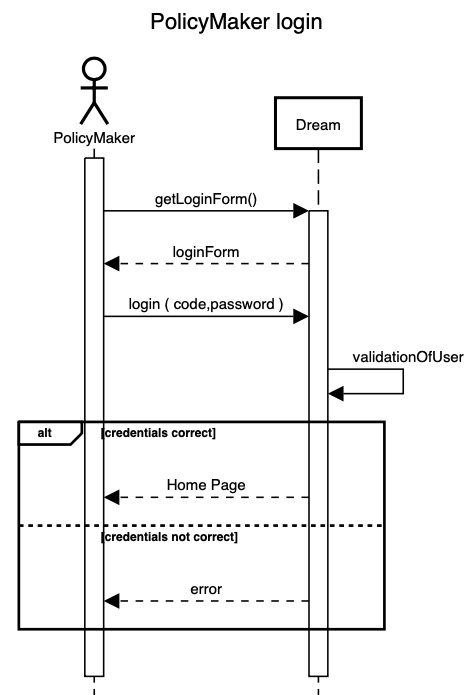
\includegraphics[width=0.7\textwidth]{sequence/PolicyMakerLogin.png}
        \caption{\emph{Policy Maker login} sequence diagram}
        \label{fig:sequence9}
        \end{center}
    \end{figure}

    \item Find a farm's page
    \begin{longtable}{p{0.26\linewidth}p{0.75\linewidth}}
        \toprule
        \textbf{Name} & \textbf{Policy Maker visualizes a farm’s page} \\
        \midrule
        \textbf{Actors} & Policy Maker \\
        \midrule
        \textbf{Entry conditions} & The Policy Maker has logged in\\
        \midrule
        \textbf{Flow of events} & 
        \begin{enumerate}
            \item The Policy Maker wants to visualize one farm's page
            \item The Policy Maker type the name of the farm on the search form
            \item The Policy Maker clicks search button
            \item The system redirect the Policy Maker to the farm's page
        \end{enumerate} \\
        \midrule
        \textbf{Exit conditions} & The Policy Maker visualizes the farm's page\\
        \midrule
        \textbf{Exceptions} & 
        \begin{itemize}
            \item If no name is inserted in the search form the system notifies the Policy Maker of the missing data
            \item If the name inserted is not found by the system in the database, it send an error message
        \end{itemize}\\
        \bottomrule
        \caption{\emph{Farm’s page visualization} use case description}
    \end{longtable}
    \begin{figure}[H]
        \begin{center}
        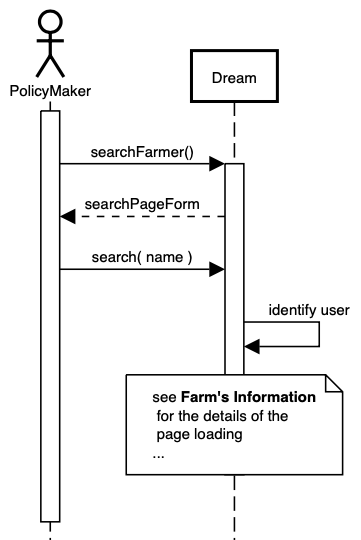
\includegraphics[width=0.7\textwidth]{sequence/PolicyMakerseachFarm.png}
        \caption{\emph{Farm’s page visualization} sequence diagram}
        \label{fig:sequence10}
        \end{center}
    \end{figure}

    \item Find a farmer on the Map
    \begin{longtable}{p{0.26\linewidth}p{0.75\linewidth}}
        \toprule
        \textbf{Name} & \textbf{Policy Maker visualizes a farm’s page} \\
        \midrule
        \textbf{Actors} & Policy Maker \\
        \midrule
        \textbf{Entry conditions} & The Policy Maker has logged in\\
        \midrule
        \textbf{Flow of events} & 
        \begin{enumerate}
            \item The Policy Maker wants to visualize the map
            \item The Policy Maker clicks on map button
            \item The system redirect the Policy Maker to the map page
            \item The Policy Maker visualizes the map and select a farm
            \item The system retrieves the information about the farm (also the last evaluation) and shows them to the Policy Maker
            \item The Policy Maker visualizes the data about the selected farm
        \end{enumerate} \\
        \midrule
        \textbf{Exit conditions} & The Policy Maker visualizes his own data\\
        \midrule
        \textbf{Exceptions} & 
        \begin{itemize}
            \item 
        \end{itemize}\\
        \bottomrule
        \caption{\emph{Farm visualization on map} use case description}
    \end{longtable}
    \begin{figure}[H]
        \begin{center}
        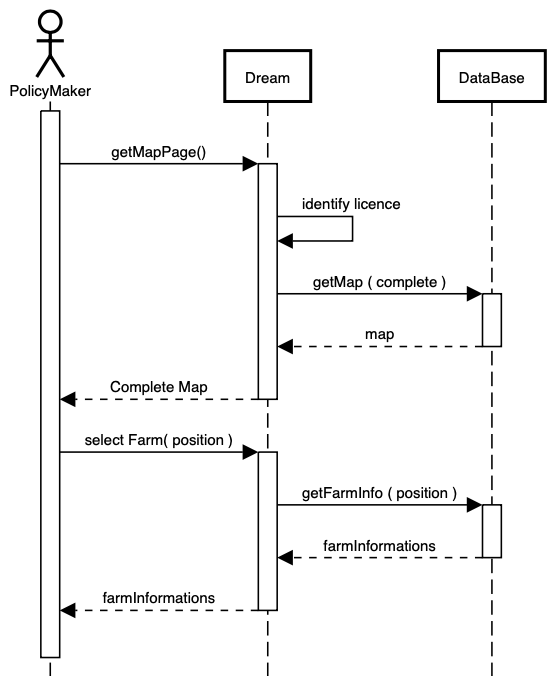
\includegraphics[width=0.7\textwidth]{sequence/searchOnMap.png}
        \caption{\emph{Farm visualization on map} sequence diagram}
        \label{fig:sequence11}
        \end{center}
    \end{figure}

    \item Update the Map
    \begin{longtable}{p{0.26\linewidth}p{0.75\linewidth}}
        \toprule
        \textbf{Name} & \textbf{Policy Maker update the map} \\
        \midrule
        \textbf{Actors} & Policy Maker \\
        \midrule
        \textbf{Entry conditions} & The Policy Maker has logged in\\
        \midrule
        \textbf{Flow of events} & 
        \begin{enumerate}
            \item The Policy Maker wants to report an evaluation
            \item The Policy Maker clicks on map button
            \item The system redirect the Policy Maker to the map page
            \item The Policy Maker visualizes the map and select a farm
            \item The system retrieves the information about the farm (also the last evaluation) and shows them to the Policy Maker
            \item The Policy Maker clicks update button
            \item The Policy Maker select the evaluation
                \begin{itemize}
                    \item The Policy Maker select "good" , an amount of money for the award and writes the body of the message
                    \item The Policy Maker select "bad" and writes the body of the message
                \end{itemize}
            \item The Policy Maker clicks submit button and send the message
            \item The system save the evaluation on the map
            \item The system send the message to the Fram's owner
            \item The system notifies the Policy Maker that the operation went succesfully 
        \end{enumerate} \\
        \midrule
        \textbf{Exit conditions} & The Policy Maker visualizes the map updated\\
        \midrule
        \textbf{Exceptions} & 
        \begin{itemize}
            \item 
        \end{itemize}\\
        \bottomrule
        \caption{\emph{Map updating} use case description}
    \end{longtable}
    \begin{figure}[H]
        \begin{center}
        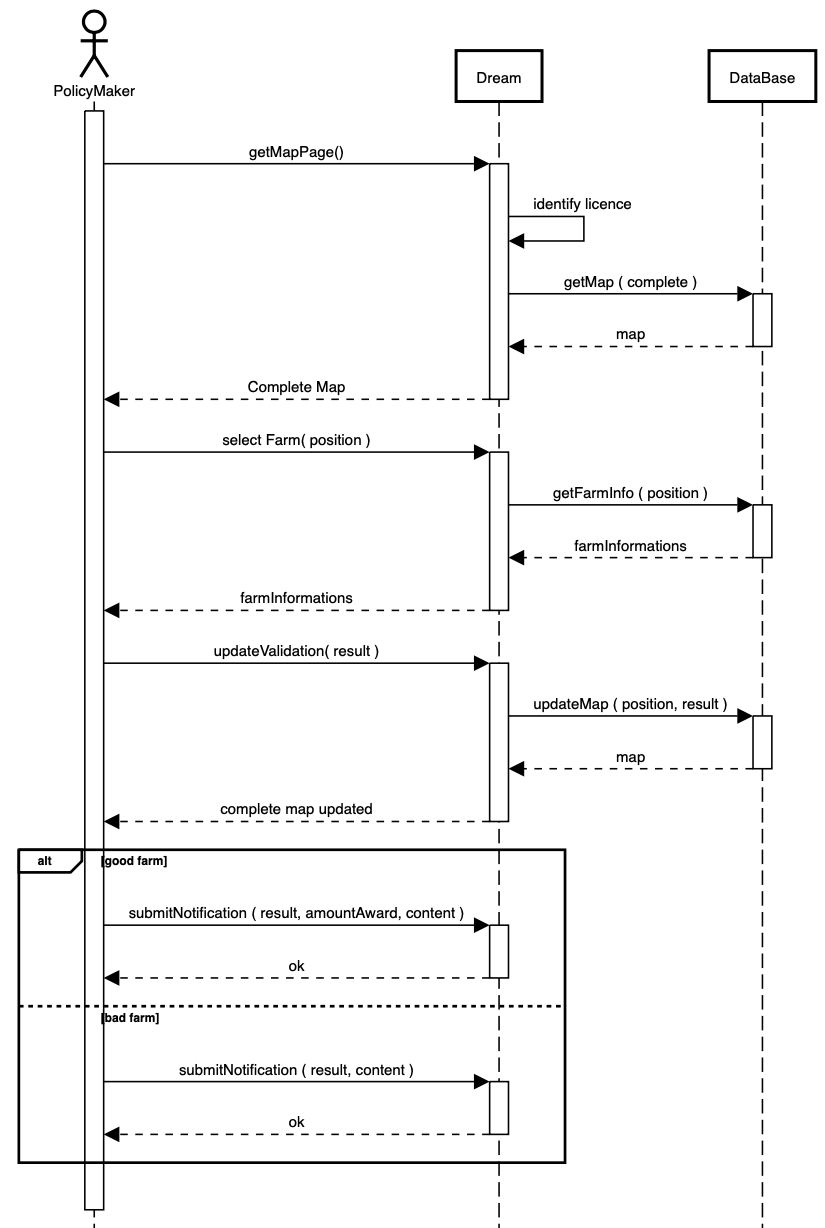
\includegraphics[width=0.7\textwidth]{sequence/updateMap.png}
        \caption{\emph{Map updating} sequence diagram}
        \label{fig:sequence12}
        \end{center}
    \end{figure}

    \item Reply to a request of help
    \begin{longtable}{p{0.26\linewidth}p{0.75\linewidth}}
        \toprule
        \textbf{Name} & \textbf{Policy Maker send anvice} \\
        \midrule
        \textbf{Actors} & Policy Maker \\
        \midrule
        \textbf{Entry conditions} & The Policy Maker has logged in\\
        \midrule
        \textbf{Flow of events} & 
        \begin{enumerate}
            \item The Policy Maker wants to send specific advices to a farmer
            \item The Policy Maker wants to see the farm's farm information
            \item The Policy Maker type the name of the farm on search form
            \item The Policy Maker clicks search button 
            \item The Policy Maker wants to see the advices stored in the database on the type of production the farmers ask for help on
            \item The Policy Maker analyze the data 
            \item The Policy Maker select the farmer ( addressee ),the type of production and writes the solution he found
            \item The Policy Maker clicks send button
            \item The system sends the message to the farmer
            \item The system notifies the Policy Maker that the operation went succesfully
        \end{enumerate} \\
        \midrule
        \textbf{Exit conditions} & The Policy Maker send solutions\\
        \midrule
        \textbf{Exceptions} & 
        \begin{itemize}
            \item 
        \end{itemize}\\
        \bottomrule
        \caption{\emph{Problem resolution} use case description}
    \end{longtable}
    \begin{figure}[H]
        \begin{center}
        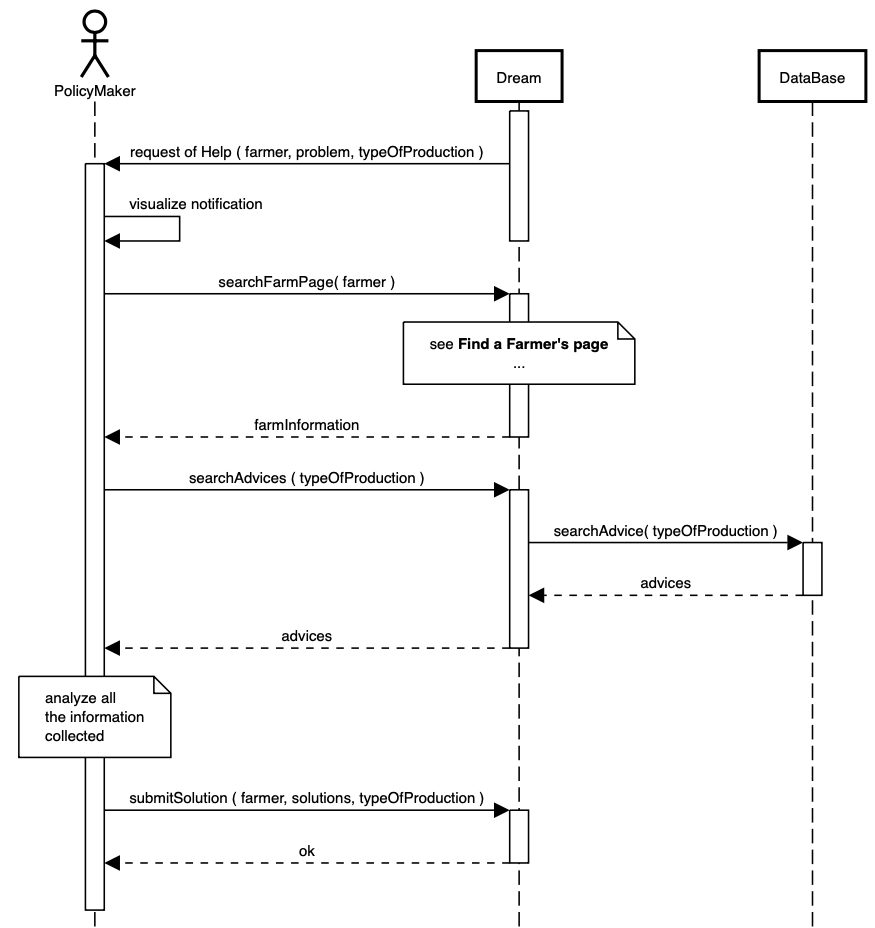
\includegraphics[width=0.7\textwidth]{sequence/replyHelp.png}
        \caption{\emph{Problem resolution} sequence diagram}
        \label{fig:sequence13}
        \end{center}
    \end{figure}
\end{enumerate}

%-----------------------------------------------------------------------------------%
\subsubsection{Scenarios}
\begin{enumerate}
    \item \textbf{Scenario 1}
    Dayanita is a young woman that lives in Singaram, a small town in the region of Telengana in India
    \item 
\end{enumerate}


%-----------------------------------------------------------------------------------%
\subsubsection{Requirements}
\textbf{R1} the system must allow farmers to register\\
\textbf{R2} the system must allow farmers to log in\\
\textbf{R3} the system must save the farmers registration data\\
\textbf{R4} the system must guarantee that each email address is unique\\
\textbf{R5} the system must verify that the email address is valid (the type!)\\
\textbf{R6} the system must save the farmers information about their production submitted\\
\textbf{R7} the system must allow farmers to insert the type of production \\
\textbf{R8} the system must allow farmers to insert the amount of production type\\
\textbf{R9} the system must allow farmers to specify a problem they faced to the Policy Makers\\
\textbf{R10} the system must allow farmers to select the type of production on which they had troubles\\
\textbf{R11} the system must save the advice submitted by the farmers\\
\textbf{R12} the system must allow farmers to select the type of product in their suggestion\\
\textbf{R13} the system must be able to show to the farmers advices send by the Policy Makers (as a notification)\\
\textbf{R14} the system must be able to show the meteorological data of the Farm’s position\\
\textbf{R15} the system must be able to show the farm’s sensor data \\
\textbf{R16} the system must allow farmers to send messages on the forum\\
\textbf{R17} the system must register date and time of a message in the forum\\
\textbf{R18} the system must be able to show all the messages on the forum\\
\textbf{R19} the system must be able to show the map of the zone\\
\textbf{R20} the system must be able to show the farms position on the map\\
\textbf{R21} the system must be able to show on the map if a farm is performing well or not \\
\textbf{R22} the system must allow farmers to visualise notification send by Policy Makers\\
\textbf{R23} the system does not allow Policy Makers to register\\
\textbf{R24} the system must allow Policy Makers to log in\\
\textbf{R25} the system must allow Policy Makers to search a farm by name (OK?)\\
\textbf{R26} the system must allow Policy Makers to see all farms’ pages\\
\textbf{R27} the system must not allow Policy Makers to modify any farm’s page\\
\textbf{R28} the system must allow Policy Makers to update the performance of a farmer\\
\textbf{R29} the system must allow Policy Makers to send notification to the farmers\\
\textbf{R30} the system must allow Policy Makers to receive request of help by the farmers\\
%-----------------------------------------------------------------------------------%
\subsubsection{Goals}
\begin{itemize}   
\item \textbf{G1} Allow Policy Makers to retrieve information about a farm
    \begin{itemize}
        \renewcommand\labelitemi{--}
        \item \textbf{R14} The system must be able to show the meteorological data of the Farm’s position
        \item \textbf{R15} The system must be able to show the farm’s sensor data
        \item \textbf{R23} The system does not allow Policy Makers to register
        \item \textbf{R24} The system must allow Policy Makers to log in
        \item \textbf{} The system must verify that the code is valid
        \item \textbf{R25} The system must allow Policy Makers to search a farm by name
        \item \textbf{R26} The system must allow Policy Makers to see all farms’ pages
        \item \textbf{R27} The system must not allow Policy Makers to modify any farm’s page
        \item \textbf{}
        \item \textbf{}
        \item \textbf{}
        \item \textbf{}
        \item \textbf{}
        \item \textbf{}
    \end{itemize}

\item \textbf{G2} Allow farmer to comunicate with each other
    \begin{itemize}
        \renewcommand\labelitemi{--}
        \item \textbf{R1} The system must allow farmers to register
        \item \textbf{R2} The system must allow farmers to log in
        \item \textbf{R3} The system must save the farmers registration data
        \item \textbf{R4} The system must guarantee that each email address is unique
        \item \textbf{R5} The system must verify that the email address is valid
        \item \textbf{R16} The system must allow farmers to send messages on the forum
        \item \textbf{R17} The system must register date and time of a message in the forum
        \item \textbf{R18} The system must be able to show all messages on the forum
    \end{itemize}    

\item \textbf{G3} Allow farmer to insert data and advices on his production
    \begin{itemize}
    \renewcommand\labelitemi{--}
    \item \textbf{R1} The system must allow farmers to register
    \item \textbf{R2} The system must allow farmers to log in
    \item \textbf{R3} The system must save the farmers registration data
    \item \textbf{R4} The system must guarantee that each email address is unique
    \item \textbf{R5} The system must verify that the email address is valid
    \item \textbf{R6} The system must save the farmers information about their production submitted
    \item \textbf{R7} The system must allow farmers to insert the type of production
    \item \textbf{R8} The system must allow farmers to insert the amount of production type
    \item \textbf{R11} The system must save the advice submitted by the farmers
    \item \textbf{R12} The system must allow farmers to select the type of product in their suggestion
    \item \textbf{}
    \end{itemize} 

\item \textbf{G4} Allow farmer to send request of help to Policy Makers
    \begin{itemize}
    \renewcommand\labelitemi{--}
    \item \textbf{R1} The system must allow farmers to register
    \item \textbf{R2} The system must allow farmers to log in
    \item \textbf{R3} The system must save the farmers registration data
    \item \textbf{R4} The system must guarantee that each email address is unique
    \item \textbf{R5} The system must verify that the email address is valid
    \item \textbf{R9} The system must allow farmers to specify a problem they faced to the Policy Makers
    \item \textbf{R10} The system must allow farmers to select the type of production on which they had troubles
    \item \textbf{R13} The system must be able to show to the farmers advices send by the Policy Makers
    \item \textbf{R22} The system must allow farmers to visualise notification send by Policy Makers
    \item \textbf{R29} The system must allow Policy Makers to send notification to the farmers
    \item \textbf{R30} The system must allow Policy Makers to receive request of help by the farmers
    \item \textbf{}
    \item \textbf{}
    \item \textbf{}
    \item \textbf{}
    \item \textbf{}
    \end{itemize} 

\item \textbf{G5} The impact of meteorological data on farmer activity can be used for further information
    \begin{itemize}
    \renewcommand\labelitemi{--}
    \item \textbf{R14} The system must be able to show the meteorological data of the Farm’s position
    \item \textbf{R26} The system must allow Policy Makers to see all farms’ pages
    \item \textbf{R28} The system must allow Policy Makers to update the performance of a farmer
    \item \textbf{}
    \item \textbf{}
    \item \textbf{}
    \item \textbf{}
    \item \textbf{}
    \item \textbf{}
    \item \textbf{}
    \item \textbf{}
    \end{itemize} 

\item \textbf{G6} Allow farmers to retrieve information relevant for their activity
    \begin{itemize}
    \renewcommand\labelitemi{--}
    \item \textbf{R1} The system must allow farmers to register
    \item \textbf{R2} The system must allow farmers to log in
    \item \textbf{R3} The system must save the farmers registration data
    \item \textbf{R4} The system must guarantee that each email address is unique
    \item \textbf{R5} The system must verify that the email address is valid
    \item \textbf{R14} The system must be able to show the meteorological data of the Farm’s position
    \item \textbf{R15} The system must be able to show the farm’s sensor data
    \item \textbf{} The system must allow farmers to their own Farm's page
    \item \textbf{R22} The system must allow farmers to visualise notification send by Policy Makers
    \item \textbf{}
    \item \textbf{}
    \item \textbf{}
    \item \textbf{}
    \item \textbf{}
    \item \textbf{}
    \item \textbf{}
    \end{itemize} 
    
\item \textbf{G7} Policy Makers and farmers should be able to consult the map of the zone ( and the informations stored in it ) with different levels of visibility\\
    \begin{enumerate}
        \item \textbf{G7A} Policy Makers and farmers should be able to see the position of the farms on the map
        \begin{itemize}
            \renewcommand\labelitemi{--}
            \item\textbf{R1} The system must allow farmers to register\\
            \item\textbf{R2} The system must allow farmers to log in\\
            \item\textbf{R3} The system must save the farmers registration data\\
            \item\textbf{R4} The system must guarantee that each email address is unique\\
            \item\textbf{R5} The system must verify that the email address is valid\\
            \item\textbf{R19} The system must be able to show the map of the zone\\
            \item\textbf{R20} The system must be able to show the farms position on the map\\
            \item\textbf{R23} The system does not allow Policy Makers to register\\
            \item\textbf{R24} The system must allow Policy Makers to log in\\
            \item\textbf{} The system must verify that the code is valid\\
            \item\textbf{}
            \item\textbf{}
            \item\textbf{}
        \end{itemize}
        \item\textbf{G7B} Policy Makers should be able to see both the information about the production and the evaluation of each farm
        \begin{itemize}
            \renewcommand\labelitemi{--}
            \item \textbf{} The system must be able to show the types of production cultivated in a farm\\
            \item \textbf{} The system must be able to show the quantity of product has been cultivated for each type and farm\\
            \item \textbf{R19} The system must be able to show the map of the zone\\
            \item \textbf{R20} The system must be able to show the farms position on the map\\
            \item \textbf{R21} The system must be able to show on the map if a farm is performing well or not\\
            \item \textbf{R23} The system does not allow Policy Makers to register\\
            \item \textbf{R24} The system must allow Policy Makers to log in\\
            \item \textbf{} The system must verify that the code is valid\\
            \item \textbf{R28} The system must allow Policy Makers to update the performance of a farmer\\
            \item \textbf{R29} The system must allow Policy Makers to send notification to the farmers\\
            \item \textbf{}
            \item \textbf{}
            \item \textbf{}
            \item \textbf{}
        \end{itemize}    
        \item \textbf{G7C} Farmers should be able to see only the type of production of a farmer by the map
        \begin{itemize}
            \renewcommand\labelitemi{--}
            \item \textbf{R1} The system must allow farmers to register\\
            \item \textbf{R2} The system must allow farmers to log in\\
            \item \textbf{R3} The system must save the farmers registration data\\
            \item \textbf{R4} The system must guarantee that each email address is unique\\
            \item \textbf{R5} The system must verify that the email address is valid\\
            \item \textbf{} The system must be able to show the types of production cultivated in a farm\\
            \item \textbf{R19} The system must be able to show the map of the zone\\
            \item \textbf{R20} The system must be able to show the farms position on the map\\
            \item \textbf{}
            \item \textbf{}
            \item \textbf{}
            \item \textbf{}
            \item \textbf{}
            \item \textbf{}
            \item \textbf{}
        \end{itemize}
    \end{enumerate}
\end{itemize}
    
\textbf{}
    \textbf{}
    \textbf{}
    \textbf{}
    \textbf{}
    \textbf{}
    \textbf{}
    \textbf{}
    \textbf{}
    \textbf{}
    \textbf{}
    \textbf{}



%-----------------------------------------------------------------------------------%
\subsubsection{Traceability Matrix}
%-----------------------------------------------------------------------------------%
\subsection{Performance Requirements}
The system serves its user with a web application. All the computations will take place on the server side, 
thus the app is meant to be lightweighted. Moreover the load in the night is expected to be really low.
There are no problems about reliability. The insertion of new data requires a quick response in order to store 
it in the system.

%-----------------------------------------------------------------------------------%
\subsection{Design Constraints}
\subsubsection{Standards Compliance}
The only standard that needs to be highlighted here is the interaction with the database. It is important that the information are stored 
in a standardized form. In such manner, it is easier to memorize and retrieve data.


\subsubsection{Any Other Constraints}
Interaction between Dream and users needs to consider also regulatory policies.
As a matter of fact the application asks and retrieves data of each farmer.
More information about security and privacy will be provided in the section~\ref{subsubsection:3.4.3}


%-----------------------------------------------------------------------------------%
\subsection{Software System Attributes}

\subsubsection{Reliability}
The system must prevent any failure in order to guarantee continuity. 
Simultaneous accesses are expected to work, especially in the afternoon when users are expectd to insrt and retrieve more information.

\subsubsection{Availability}
It is expected that the system has the lowest downtime possible. 
The system is available with a minimum time of 96\%, 
so that it about 14 days a year of downtime are allowed.


\subsubsection{Security}
\label{subsubsection:3.4.3}
Security of the data and of the communication user-system is a primary concern. Users credential are stored in a data base, so the system crypt the password data before store it. The system recognises the right type of user during the log in phase to ensure providing the correct level visibility of the data and the permission to update them or not. In this way farmer’s privacy is guaranteed. As a matter of fact a farmer can’t see another farmer’s page.


\subsubsection{Maintanability}
The web application requires ordinary maintenance for improvements and in order to fix potential bugs. 
It is going to be scheduled at local night time, when user traffic is the lowest.
Moreover the system must be designed in a way that allows future addition of features.

\subsubsection{Portability}
The system as a web application must run on different software system as Windows, Linux an macOS.
On the server side is crucial focusing on the interaction between APIs and the data base to insert, update or read data.

